\documentclass[12pt]{article}
\usepackage[utf8]{inputenc}
\usepackage{lmodern}
\usepackage[T1]{fontenc}
\usepackage{amsmath}
\usepackage{enumitem}
\usepackage{graphicx}
\usepackage{fullpage}
\usepackage{siunitx}
\usepackage{fancyhdr}
\PassOptionsToPackage{hyphens}{url}
\usepackage[hyphens]{url}
\usepackage{color}
\usepackage{enumitem}
\usepackage{textcomp}
\usepackage{geometry}
\usepackage{courier}
\usepackage{listings}
\usepackage{array}
\usepackage{amsthm}
\usepackage{mathdots}
\usepackage{amssymb}
\usepackage{minted}
\usepackage{wrapfig}
\usepackage{titlesec}
\usepackage{parskip}
\usepackage{accents}
\usepackage{gensymb}
\usepackage{indentfirst}
\usepackage{courier}
\usepackage{framed}
\usepackage{etoolbox}
\usepackage{titlesec}
\usepackage{appendix}
\usepackage{mdframed}
\usepackage{verbatim}
\usepackage{xspace}
\usepackage{hyperref}
\AtBeginEnvironment{subappendices}{%
\section*{Appendix}
\addcontentsline{toc}{section}{Appendices}
}



\newcommand{\mytitle}{\textbf{inzva Algorithm Programme 2018-2019\\ \ \\Bundle 4 \\ \ \\ Graph-1}}
\title{\vspace{-2em}\mytitle\vspace{-0.3em}}
\author{\textbf{Editor}\\Kayacan Vesek\\ \ \\ \textbf{Reviewer} \\Yasin Kaya}





%\lstset{language=C++,
%                basicstyle=\ttfamily,
%                keywordstyle=\color{blue}\ttfamily,
%                stringstyle=\color{red}\ttfamily,
%                commentstyle=\color{green}\ttfamily,
%                morecomment=[l][\color{magenta}]{\#}
%}

\definecolor{keywordcolor}{rgb}{0,0,0.45}
\definecolor{stringcolor}{rgb}{0.45,0.45,0.45}
\definecolor{commentcolor}{rgb}{0,0.3,0}

\lstset{
language=C++,
basicstyle=\footnotesize\ttfamily,
numbers=left,
%numberstyle=\tiny,
frame=tb,
columns=fullflexible,
showstringspaces=false,
breaklines=true,
tabsize=4,
keywordstyle=\color{keywordcolor}\footnotesize\bf\ttfamily,
stringstyle=\color{stringcolor}\footnotesize\ttfamily,
commentstyle=\color{commentcolor}\it\sffamily
}
% \lstset{basicstyle=\ttfamily,breaklines=true}
\lstloadlanguages{C++}

%\renewcommand{\familydefault}{\sfdefault}

\addtolength{\parskip}{\baselineskip}  
\newcommand{\urlwofont}[1]{\urlstyle{same}\url{#1}}

\renewcommand{\arraystretch}{0.8}
\renewcommand{\headrulewidth}{0pt}
\renewcommand{\footrulewidth}{0pt}

\newcommand{\imagewidth}{0.8\textwidth}

\lhead{}
\chead{}
\rhead{}
\lfoot{}
\cfoot{\thepage}
\rfoot{}

\geometry{
  top=0.9in,
  inner=0.7in,
  outer=0.7in,
  bottom=0.9in,
  headheight=2ex,
  headsep=1ex,
}
\pagestyle{fancy}
%\fancyhf{}
%\setlength{\headsep}{0.2in}


\fancypagestyle{firststyle}
{
    \chead{}
    \setlength{\headsep}{0.0in}
}
\hypersetup{
    unicode=true,
    colorlinks=true,
    linkcolor=blue,
    citecolor=black,
    filecolor=black,
    urlcolor=blue
}

\begingroup
    \makeatletter
    \@for\theoremstyle:=definition,remark,plain\do{%
        \expandafter\g@addto@macro\csname th@\theoremstyle\endcsname{%
            \addtolength\thm@preskip\parskip
            }%
        }
\endgroup

\newtheorem{thm}{Theorem}[section]
\newtheorem{lemma}{Lemma}[section]
\newtheorem{claim}{Claim}[section]
\newtheorem{proposition}{Proposition}[section]
%\theoremstyle{empty}
\newtheorem*{namedthm}{Theorem}


% indention size
%\setlength{\parindent}{19pt}
\setlength{\parindent}{0pt}

% paragraph spacing
\setlength{\parskip}{1em}

% line spacing
\linespread{1}

%\setcounter{tocdepth}{1}

\date{}
\begin{document}

\begin{figure}
  \centering
  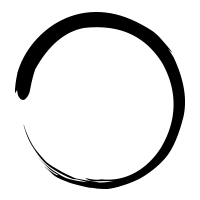
\includegraphics[width=\linewidth/4]{inzva-logo.png}
  \label{fig:inzva}
\end{figure}
\maketitle

\cleardoublepage
\tableofcontents
\markboth{Table of Contents}{}
\cleardoublepage
\newcommand{\sectionbreak}{\clearpage}

\section{Introduction}

A graph is a structure amounting to a set of objects in which some pairs of the objects are in some sense "related". The objects correspond to the mathematical abstractions called vertices (also called nodes or points) and each of the related pairs of vertices is called an edge. Typically, a graph is depicted in diagrammatic form as a set of dots for the vertices, joined by lines for the edges. \cite{1}

Why graphs? Graphs are usually used to represent different elements that are somehow related to each other.

A Graph consists of a finite set of vertices(or nodes) and set of edges which connect a pair of nodes. 

G = (V,E)

V = set of nodes

E = set of edges(e) represented as e = {a,b}

Graph are used to show a relation between objects. So, some graphs may have directional edges (e.g. people and their love relationships that are not mutual: Alice may love Alex, while Alex is not in love with her and so on), and some graphs may have weighted edges (e.g. people and their relationship in the instance of a debt)

\begin{figure}[h]
\centering
  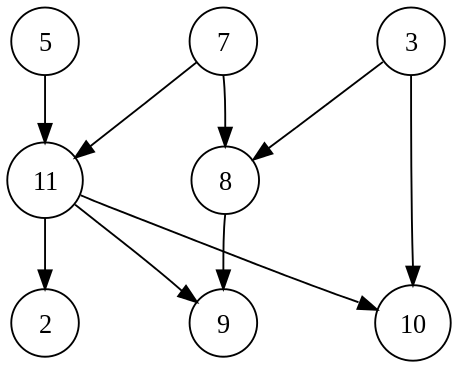
\includegraphics[width=\linewidth/2]{458px-Directed_acyclic_graph_2.png}
  
\caption{a simple unweigted graph}
\end{figure}

\section{Definitions}
    \subsection{Definitions of Common Terms}
        \begin{itemize}
          \item \texttt{Node} - An individual data element of a graph is called Node. Node is also known as vertex.
          \item \texttt{Edge} - An edge is a connecting link between two nodes. It is represented as e = {a,b} Edge is also called Arc. 
          \item \texttt{Adjacent} - Two vertices are adjacent if they are connected by an edge.
          \item \texttt{Degree} - a degree of a node is the number of edges incident to the node.  
          \item \texttt{Undirected Graphs} - Undirected graphs have edges that do not have a direction. The edges indicate a two-way relationship, in that each edge can be traversed in both directions.  
          \item \texttt{Directed Graphs} - Directed graphs have edges with direction. The edges indicate a one-way relationship, in that each edge can only be traversed in a single direction.  
          \item \texttt{Weighted Edges} - If each edge of graphs has an association with a real number, this is called its weight. 
          \item \texttt{Self-Loop} - It is an edge having the same node for both destination and source point.
          \item \texttt{Multi-Edge} - Some Adjacent nodes may have more than one edge between each other.
          
    
        \end{itemize}
        \newpage
    \subsection{Walks, Trails, Paths, Cycles and Circuits}
        \begin{itemize}
          \item \texttt{Walk} - A sequence of nodes and edges in a graph.
          
          \item \texttt{Trail} - A walk without visiting the same edge.
          
          \item \texttt{Circuit} - A trail that has the same node at the start and end.
          
          \item \texttt{Path} - A walk without visiting same node.
          
          \item \texttt{Cycle} - A circuit without visiting same node. 
          
        \end{itemize}
    \subsection{Special Graphs}
        \begin{itemize}
         \item \texttt{Complete Graph} -  A graph having at least one edge between every two nodes.
         \item \texttt{Connected Graph} -  A graph with paths between every pair of nodes. 
         \item \texttt{Tree} - an undirected connected graph that has any two nodes that are connected by exactly one path.
         There are some other definitions that you can notice it is tree:
             \begin{itemize}
             \item \texttt an undirected graph is connected and has no cycles.
             an undirected graph is acyclic, and a simple cycle is formed if any edge is added to the graph.
             \item \texttt an undirected graph is connected, it will become disconnected if any edge is removed.
             \item \texttt an undirected graph is connected, and has  (number of nodes - 1) edges.
             \end{itemize}
        \end{itemize}



\section{Representing graphs}
    \subsection{Edge lists}
        A simple way to define edge list is that it has a list of pairs. We just have a list of objects consisting of the vertex numbers of 2 nodes and other attributes like weight or the direction of edges. \cite{16}
        \begin{itemize}
             \item \texttt + For some specific algorithms you need to iterate over all the edges, (i.e. kruskal's algorithm)
             \item \texttt + All edges are stored exactly once.
             \item \texttt - It is hard to determine whether two nodes are connected or not.
             \item \texttt - It is hard to get information about the edges of a specific vertex.
         \end{itemize}
    \begin{minted}[frame=lines,linenos,fontsize=\footnotesize]{c++}
    #include <iostream>
    #include <vector>
    using namespace std;
    
    int main(){
        int edge_number;
        vector<pair <int,int> > edges;
        cin >> edge_number;
        for( int i=0 ; i<edge_number ; i++ ){
            int a,b;
            cin >> a >> b;
            edges.push_back(make_pair(a,b)); // a struct can be used if edges are weighted or have other properties.
        }
    }
    \end{minted}
    \subsection{Adjacency Matrices}
        Stores edges, in a 2-D matrix. matrix[a][b] keeps an information about road from a to b. \cite{16}
        \begin{itemize}
             \item \texttt + We can easily check if there is a road between two vertices.
             \item \texttt - Looping through all edges of a specific node is expensive because you have to check all of the empty cells too. Also these empty cells takes huge memory in a graph which has many vertices.(For example representing a tree)
         \end{itemize}
        \begin{minted}[frame=lines,linenos,fontsize=\footnotesize]{c++}
        #include <iostream>
        #include <vector>
        using namespace std;
        int main(){
            int node_number;
            vector<vector<int> > Matrix;
            cin >> node_number;
            for( int i=0 ; i<node_number ; i++ )
                for( int j=0 ; j<node_number ; j++ ){
                    Matrix.push_back(vector <int> ());
                    int weight;
                    cin >>weight ;
                    Matrix[i].push_back(weight);
                }
        }
        \end{minted}
    \subsection{Adjacency List}
    Each node has a list consisting of nodes each is adjacent to. So, there will be no empty cells. Memory will be equal to number of edges. The most used one is in algorithms. \cite{16}
        \begin{itemize}
             \item \texttt + You do not have to use space for empty cells, 
    
             \item \texttt + Easily iterate over all the neighbors of a specific node.
             \item \texttt - If you want to check if two nodes are connected, in this form you still need to iterate over all the neighbors of one of them. But, there are some structures that you can do this operation in O(log N). For example if you won't add any edge, you can sort every vector with nodes' names, so you can find it by binary search.  
            
         \end{itemize} 
        \begin{minted}[frame=lines,linenos,fontsize=\footnotesize]{c++}
        #include <iostream>
        #include <vector>
        using namespace std;
        
        int main(){
            int node_number,path_number;
            
            vector<vector<int> > paths; 
            // use object instead of int, 
            //if you need to store other features
            
            cin >> node_number >> path_number;
            for( int i=0 ; i<node_number ; i++ )
                Matrix.push_back(vector <int> ());
            for( int j=0 ; j< path_number ; j++ ){
                int  beginning_node,end_node;
                cin >> beginning_node >> end_node;
                
                Matrix[ beginning_node ].push_back( end_node ); // push st
                // Matrix[ end_node ].push_back(  beginning_node ); 
                // ^^^ If edges are Undirected, you should push in reverse direction too
            }
        }
        \end{minted}
\section{Tree Traversals}
     The tree traversal is the process of visiting every node exactly once in a tree structure  for some purposes(like getting information or updating information). In a binary tree there are some described order to travel, these are specific for binary trees but they may be generalized to other trees and even graphs as well. \cite{Traversal}



        \begin{figure}
        \centering
      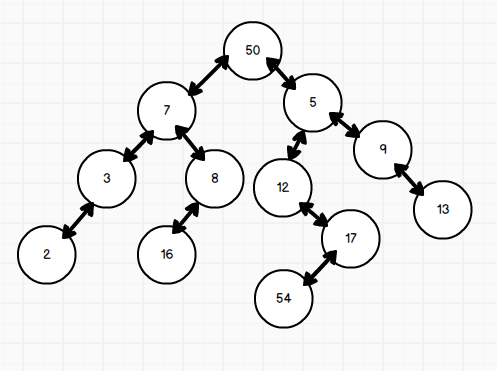
\includegraphics[width=\linewidth/3*2]{binary-tree.png}

        \caption{a binary tree}
    \end{figure}
    \newpage
    \subsection{Preorder}
    Preorder means that a root will be evaluated before its children. In other words the order of evaluation is: Root-Left-Right
    \begin{itemize}
     \item \texttt Preorder
     \item \texttt 1. Look Data
     \item \texttt 2. Traverse the left node
     \item \texttt 3. Traverse the right node 
     \item \texttt Example:  50 – 7 – 3 – 2 – 8 – 16 – 5 – 12 – 17 – 54 – 9 – 13
    \end{itemize}
    \subsection{Inorder}
    Inorder means that the left child (and all of the left child’s children) will be evaluated before the root and before the right child and its children. Left-Root-Right (by the way, in binary search tree inorder retrieves data in sorted order)
    \begin{itemize}
     \item \texttt Inorder
     \item \texttt 1. Traverse the left node
     \item \texttt 2. Look Data
     \item \texttt 3. Traverse the right node 
     \item \texttt Example:  2 – 3 – 7 – 16 – 8 – 50 – 12 – 54 – 17 – 5 – 9 – 13
    \end{itemize}
    \subsection{Postorder}
    Postorder is the opposite of preorder, all children are evaluated before their root: Left-Right-Root
    \begin{itemize}
     \item \texttt Postorder
     \item \texttt 1. Traverse the left node
     \item \texttt 2. Traverse the right node 
     \item \texttt 3. Look Data
     \item \texttt Example: 2 – 3 – 16 – 8 – 7 – 54 – 17 – 12 – 13 – 9 – 5 – 50
    \end{itemize}
\subsection{Implementation}
 \begin{minted}[frame=lines,linenos,fontsize=\footnotesize]{python3}
class Node: 
    def __init__(self,key): 
        self.left = None
        self.right = None
        self.val = key 

def printInorder(root): 
    if root: 
        printInorder(root.left) 
        print(root.val), 
        printInorder(root.right) 
  
def printPostorder(root): 
  
    if root: 
        printPostorder(root.left) 
  
        printPostorder(root.right) 
  
        print(root.val), 
  
def printPreorder(root): 
  
    if root: 
        print(root.val), 
  
        printPreorder(root.left) 
  
        printPreorder(root.right) 
\end{minted}


\section{Binary Search Tree}
 A Binary tree is a tree data structure in which each node has at most two children, which are referred to as the left child and the right child.
 
 For a binary tree to be a binary search tree, the values of all the nodes in the left sub-tree of the root node should be smaller than the root node's value. Also the values of all the nodes in the right sub-tree of the root node should be larger than the root node's value. \cite{4,5,13}
 
  \begin{figure}[h]
  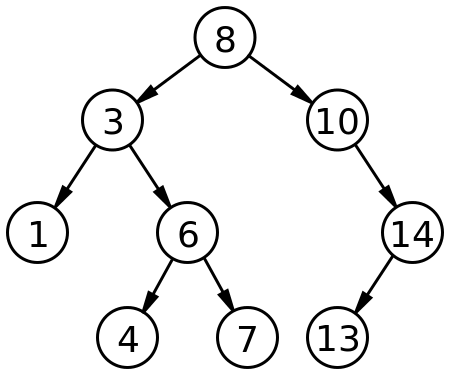
\includegraphics[width=\linewidth/2]{binarytree.png}
    \centering
    \caption{a simple binary search tree}
  \end{figure}
\subsection{Insertion Algorithm}
    \begin{itemize}
        \item Step 1: Compare values of the root node and the element to be inserted.
        
        \item Step 2: If the value of the root node is larger, and if a left child exists, then repeat step 1 with root = current root's left child. Else, insert element as left child of current root.
        
        \item Step 3: If the value of the root node is lesser, and if a right child exists, then repeat step 1 with root = current root's right child. Else, insert element as right child of current root.

    \end{itemize}



\newpage
\subsection{Deletion Algorithm}

    \begin{itemize}
        \item Deleting a node with no children: simply remove the node from the tree.
        \item Deleting a node with one child: remove the node and replace it with its child.
        \item Node to be deleted has two children: Find inorder successor of the node. Copy contents of the inorder successor to the node and delete the inorder successor.
        \item Note that: inorder successor can be obtained by finding the minimum value in right child of the node.\cite{14}
    \end{itemize}
    
\subsection{Sample Code}

 \begin{minted}[frame=lines,linenos,fontsize=\footnotesize]{python3}
// C program to demonstrate delete operation in binary search tree 
#include<stdio.h> 
#include<stdlib.h> 
  
struct node 
{ 
    int key; 
    struct node *left, *right; 
}; 
  
// A utility function to create a new BST node 
struct node *newNode(int item) 
{ 
    struct node *temp =  (struct node *)malloc(sizeof(struct node)); 
    temp->key = item; 
    temp->left = temp->right = NULL; 
    return temp; 
} 
  
// A utility function to do inorder traversal of BST 
void inorder(struct node *root) 
{ 
    if (root != NULL) 
    { 
        inorder(root->left); 
        printf("%d ", root->key); 
        inorder(root->right); 
    } 
} 
  
/* A utility function to insert a new node with given key in BST */
struct node* insert(struct node* node, int key) 
{ 
    /* If the tree is empty, return a new node */
    if (node == NULL) return newNode(key); 
  
    /* Otherwise, recur down the tree */
    if (key < node->key) 
        node->left  = insert(node->left, key); 
    else
        node->right = insert(node->right, key); 
  
    /* return the (unchanged) node pointer */
    return node; 
} 
  
/* Given a non-empty binary search tree, return the node with minimum 
   key value found in that tree. Note that the entire tree does not 
   need to be searched. */
struct node * minValueNode(struct node* node) 
{ 
    struct node* current = node; 
  
    /* loop down to find the leftmost leaf */
    while (current->left != NULL) 
        current = current->left; 
  
    return current; 
} 
  
/* Given a binary search tree and a key, this function deletes the key 
   and returns the new root */
struct node* deleteNode(struct node* root, int key) 
{ 
    // base case 
    if (root == NULL) return root; 
  
    // If the key to be deleted is smaller than the root's key, 
    // then it lies in left subtree 
    if (key < root->key) 
        root->left = deleteNode(root->left, key); 
  
    // If the key to be deleted is greater than the root's key, 
    // then it lies in right subtree 
    else if (key > root->key) 
        root->right = deleteNode(root->right, key); 
  
    // if key is same as root's key, then This is the node 
    // to be deleted 
    else
    { 
        // node with only one child or no child 
        if (root->left == NULL) 
        { 
            struct node *temp = root->right; 
            free(root); 
            return temp; 
        } 
        else if (root->right == NULL) 
        { 
            struct node *temp = root->left; 
            free(root); 
            return temp; 
        } 
  
        // node with two children: Get the inorder successor (smallest 
        // in the right subtree) 
        struct node* temp = minValueNode(root->right); 
  
        // Copy the inorder successor's content to this node 
        root->key = temp->key; 
  
        // Delete the inorder successor 
        root->right = deleteNode(root->right, temp->key); 
    } 
    return root; 
} 

\end{minted}

\subsection{Time Complexity}
The worst case time complexity of search, insert, and deletion operations is O(h) where h is the height of Binary Search Tree. In the worst case, we may have to travel from root to the deepest leaf node. The height of a skewed tree may become $N$ and the time complexity of search and insert operation may become $O(N)$. So the time complexity of establishing $N$ node unbalanced tree may become $O(N^2)$ (for example the nodes are being inserted in a sorted way). But, with random input the  expected time complexity is $O(NlogN)$.

    However, you can implement other data structures to establish Self-balancing binary search tree (which will be taught later), popular data structures that implementing this type of tree include:
    \begin{itemize}
        \item 2-3 tree
        \item AA tree
        \item AVL tree
        \item B-tree
        \item Red-black tree
        \item Scapegoat tree
        \item Splay tree
        \item Treap
        \item Weight-balanced tree
    \end{itemize}

\section{Heap}

    \begin{figure}
      \centering
      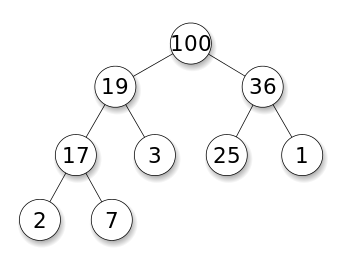
\includegraphics[width=\linewidth/2]{360px-Max-Heap.png}
     \caption{ an example max-heap with 9 nodes}
    \end{figure}
     The heap is a complete binary tree with N nodes, the value of all the nodes in the left and right sub-tree of the root node should be smaller than the root node's value. 
     
     In a heap, the highest (or lowest) priority element is always stored at the root. A heap is not a sorted structure and can be regarded as partially ordered. As visible from the heap-diagram, there is no particular relationship among nodes on any given level, even among the siblings. Because a heap is a complete binary tree, it has a smallest possible height. A heap with $N$ nodes has $logN$ height. A heap is a useful data structure when you need to remove the object with the highest (or lowest) priority. \cite{6,7}
     
     \subsection{Implementation}
     Heaps are usually implemented in an array (fixed size or dynamic array), and do not require pointers between elements. After an element is inserted into or deleted from a heap, the heap property may be violated and the heap must be balanced by internal operations.
     
     The first (or last) element will contain the root. The next two elements of the array contain its children. The next four contain the four children of the two child nodes, etc. Thus the children of the node at position n would be at positions $2*n$ and $2*n + 1$ in a one-based array. This allows moving up or down the tree by doing simple index computations. Balancing a heap is done by sift-up or sift-down operations (swapping elements which are out of order). So we can build a heap from an array without requiring extra memory.

    \begin{figure}
      \centering
      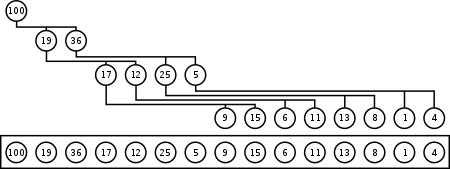
\includegraphics[width=\linewidth]{Heap-as-array.png}
     \caption{example a heap as an array}
     \label{fig:binary}
    
    \end{figure}
     
     \subsubsection{Insertion}
        Basically add the new element at the end of the heap. Then look it's parent if it is smaller or bigger depends on the whether it is max-heap or min-heap (max-heap called when Parents are always greater), swap with the parent. If it is swapped do the same operation for the parent.
        
     \subsubsection{Deletion}
        If you are going to delete a node (root node or another one does not matter), 
        \begin{itemize}
            \item Step 1:  Swap the node to be deleted with the last element of heap to maintain a balanced structure.
            \item Step 2: Delete the last element which is the node we want to delete at the start.
            \item Step 3: Now you have a node which is in the wrong place, You have to find the correct place for the swapped last element, to do this starting point you should check its left and right children, if one them is greater than our node you should swap it with the greatest child(or smallest if it is min-heap).
            \item Step 4: Still current node may in the wrong place, so apply Step 3 as long as it is not greater than its children(or smaller if it is min-heap).
        \end{itemize}
        \begin{figure}[h]
        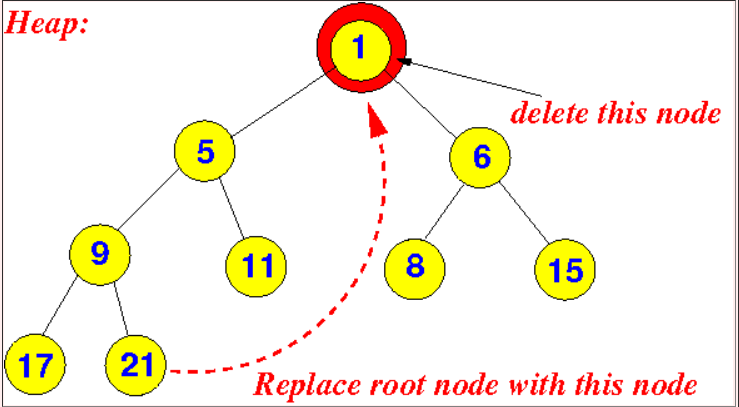
\includegraphics[width=\linewidth/2 ]{heap1.png} 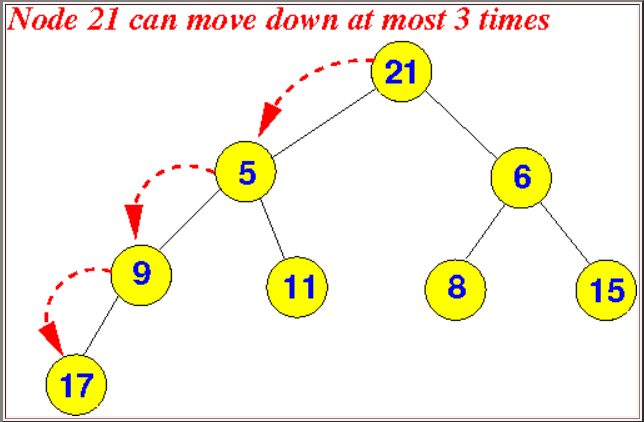
\includegraphics[width=\linewidth/2 ]{heap2.png}
        \caption{an example deletion on a heap structure}
    \end{figure}


    \begin{minted}[frame=lines,linenos,fontsize=\footnotesize]{python3}
class BinHeap:
    def __init__(self):
        self.heapList = [0]
        self.currentSize = 0


    def percUp(self,i):
        while i // 2 > 0:
          if self.heapList[i] < self.heapList[i // 2]:
             tmp = self.heapList[i // 2]
             self.heapList[i // 2] = self.heapList[i]
             self.heapList[i] = tmp
          i = i // 2

    def insert(self,k):
      self.heapList.append(k)
      self.currentSize = self.currentSize + 1
      self.percUp(self.currentSize)

    def percDown(self,i):
      while (i * 2) <= self.currentSize:
          mc = self.minChild(i)
          if self.heapList[i] > self.heapList[mc]:
              tmp = self.heapList[i]
              self.heapList[i] = self.heapList[mc]
              self.heapList[mc] = tmp
          i = mc

    def minChild(self,i):
      if i * 2 + 1 > self.currentSize:
          return i * 2
      else:
          if self.heapList[i*2] < self.heapList[i*2+1]:
              return i * 2
          else:
              return i * 2 + 1

    def delMin(self):
      retval = self.heapList[1]
      self.heapList[1] = self.heapList[self.currentSize]
      self.currentSize = self.currentSize - 1
      self.heapList.pop()
      self.percDown(1)
      return retval

    def buildHeap(self,alist):
      i = len(alist) // 2
      self.currentSize = len(alist)
      self.heapList = [0] + alist[:]
      while (i > 0):
          self.percDown(i)
          i = i - 1

bh = BinHeap()
bh.buildHeap([9,5,6,2,3])

print(bh.delMin())
print(bh.delMin())
print(bh.delMin())
print(bh.delMin())
print(bh.delMin())
\end{minted}

\subsection{Complexity}
        Insertion $O(logN)$, delete-min $O(logN)$ , and finding minimum $O(1)$. These operations depend on heap's height and heaps  are always complete binary trees, basically the height is $logN$. ( N is number of Node)
        \newpage
\subsection{Priority queue}
    Priority queues are a type of container adaptors, specifically designed so that its first element is always the greatest of the elements it contains, according to some strict weak ordering criterion.

    While priority queues are often implemented with heaps, they are conceptually distinct from heaps. A priority queue is an abstract concept like "a list" or "a map"; just as a list can be implemented with a linked list or an array, a priority queue can be implemented with a heap or a variety of other methods such as an unordered array. \cite{8,9}
    \begin{minted}[frame=lines,linenos,fontsize=\footnotesize]{c++}
#include <iostream>       // std::cout
#include <queue>          // std::priority_queue
using namespace std;
int main ()
{
  priority_queue<int> mypq;

  mypq.push(30);
  mypq.push(100);
  mypq.push(25);
  mypq.push(40);

  cout << "Popping out elements...";
  while (!mypq.empty())
  {
     cout << ' ' << mypq.top();
     mypq.pop();
  }
  return 0;
}
\end{minted}

    

\section{Depth First Search}

    Depth First Search (DFS) is an algorithm for traversing or searching tree. (For example, you can check if graph is connected or not via DFS)  \cite{15}

    \begin{figure}[h]
      \centering
         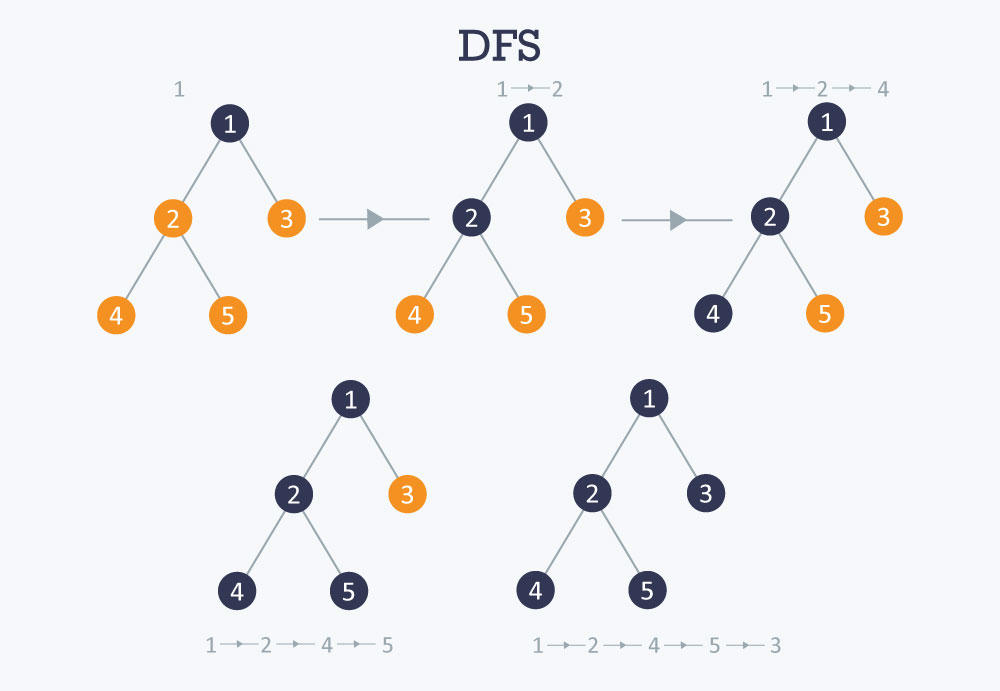
\includegraphics[width=\linewidth /3*2]{9fa1119.jpg}
     \caption{example of dfs traversal}
    \end{figure}    
    \subsection{Method}
        The DFS algorithm is a recursive algorithm that uses the idea of backtracking. It involves exhaustive searches of all the nodes by going ahead, if possible, else by backtracking.

        Here, the word backtrack means that when you are moving forward and there are no more nodes along the current path, you move backwards on the same path to find nodes to traverse. All the nodes will be visited on the current path till all the unvisited nodes have been traversed after which the next path will be selected. \cite{18}
        \begin{minted}[frame=lines,linenos,fontsize=\footnotesize]{c++}
        vector<vector<int>> adj; // graph represented as an adjacency list
        int n; // number of vertices
        vector<bool> visited;
        void dfs(int v) {
            visited[v] = true;
            for (int u : adj[v]) {
                if (!visited[u])
                    dfs(u);
            }
        }
        
        
    \end{minted}
    This recursive nature of DFS can be implemented using stacks. The basic idea is as follows:
    Pick a starting node and push all its adjacent nodes into a stack.
    Pop a node from stack to select the next node to visit and push all its adjacent nodes into a stack.
    Repeat this process until the stack is empty. However, ensure that the nodes that are visited are marked. This will prevent you from visiting the same node more than once. If you do not mark the nodes that are visited and you visit the same node more than once, you may end up in an infinite loop. \cite{18}
    
   \begin{minted}[frame=lines,linenos,fontsize=\footnotesize]{c++}
        DFS-iterative (G, s):   //Where G is graph and s is source vertex
      let S be stack
      S.push( s )   //Inserting s in stack 
      mark s as visited.
      while ( S is not empty):
          //Pop a vertex from stack to visit next
          v  =  S.top( )
         S.pop( )
         //Push all the neighbours of v in stack that are not visited   
        for all neighbours w of v in Graph G:
            if w is not visited :
                     S.push( w )         
                    mark w as visited
    \end{minted}

    
    Example Question: Given an undirected graph, find out whether the graph is strongly connected or not? An undirected graph is strongly connected if there is a path between any two pair of vertices.
    \begin{minted}[frame=lines,linenos,fontsize=\footnotesize]{c++}

#include <bits/stdc++.h>
using namespace std;

cont int MaxN=100005; // Max number of nodes

vector <int> adj[MaxN];
bool mark[MaxN];

void dfs(int k)
{
    mark[k]=1;  // visited
    
    for(auto j : adj[k]) // iterate over adjacent nodes 
        if(mark[j]==false) // check if it is visited or not
            dfs(j); // do these operation for that node
}
int main() 
{ 
    cin >> n >> m;  // number of nodes , number of edges
    for (int i=0 ; i < m; i++)
    {
        cin >> a >> b;
        adj[a].push_back(b);
        adj[b].push_back(a);
    }
    dfs(1);

    bool connected=1;
    for(int i=1 ; i <= n ;i++)
        if(mark[i]==0)
        {
            connected=0;
            break;
        }
    if(connected)
        cout << "Graph is connected" << endl;
    else
        cout << "Graph is not connected" << endl;
    return 0; 
} 
\end{minted}

\subsection{Complexity}
The time complexity of DFS is O (V+E) when implemented using an adjacency list ( with Adjacency Matrices it is  $O(V^2)$), where V is the number of nodes and E is the number of edges. \cite{2}


\section{Breadth First Search}
    Breadth First Search (BFS) is an algorithm for traversing or searching tree. (For example, you can find the shortest path fron one node to another in an unweighted graph. 
\begin{figure}[h]
    \centering
    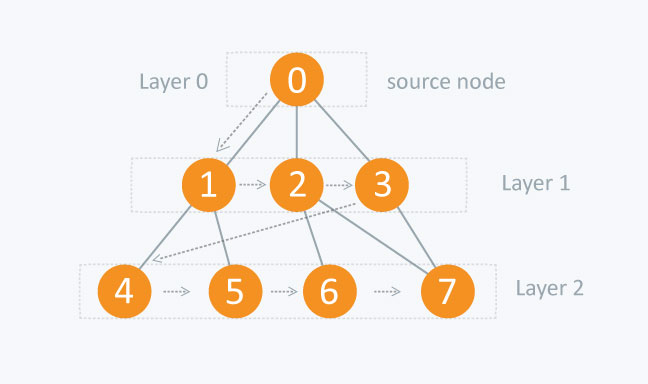
\includegraphics[width=\linewidth/2]{fdec3c2.jpg}
    \caption{An example breadth first search traversal}
    \label{fig:my_label}
\end{figure}

    \subsection{Method}
BFS is a traversing algorithm where you should start traversing from a selected node (source or starting node) and traverse the graph layerwise thus exploring the neighbour nodes (nodes which are directly connected to source node). You must then move towards the next-level neighbour nodes. \cite{3}

    \begin{itemize}
        

        \item 
        As the name BFS suggests, you are required to traverse the graph breadthwise as follows:
        \item 
        First move horizontally and visit all the nodes of the current layer
        \item 
        Add to the queue neighbour nodes of current layer.
        \item 
        Move to the next layer, which are in the queue     

        \end{itemize}

Example question: Given a unweighted graph, a source and a destination, we need to find shortest path from source to destination in the graph in most optimal way?        
    \begin{minted}[frame=lines,linenos,fontsize=\footnotesize]{c++}
#include <bits/stdc++.h>
using namespace std;

cont int MaxN=100005; // Max number of nodes

vector <int> adj[MaxN];
bool mark[MaxN];

void bfs(int starting_point,int ending_point)
{
    memset(mark,0,sizeof(mark)); //clear the cache
    queue <pair <int,int> > q; // the value of node  
    // , and length between this node and the starting node
    q.push_back(make_pair(starting_point,0));
    mark[starting_point]=1;
    while(q.empty()==false)  
    {
        pair <int,int> tmp = q.front(); // get the next node
        q.pop(); // delete from q  
        if(ending_point==tmp.first)
        {
            printf("The length of path between %d - %d : %d\n",
            starting_point,ending_point,tmp.second);
            return ;
        }
        for (auto j : adj[tmp.first])
        {
            if(mark[j]) continue ; // if it reached before
            mark[j]=1;
            q.push_back(make_pair(j,tmp.second+1)); // add next node to queue 
        }
    }
}
int main() 
{ 
    cin >> n >> m;  // number of nodes , number of edges
    for (int i=0 ; i < m; i++)
    {
        cin >> a >> b;
        adj[a].push_back(b);
    }
    cin >> start_point >> end_point;
    bfs(start_point);

    return 0; 
}
 
\end{minted}

\subsection{Complexity}
The time complexity of BFS is O(V + E), where V is the number of nodes and E is the number of edges.


\section{Union Find}
    A disjoint-set data structure is a data structure that keeps track of a set of elements partitioned into a number of disjoint (non-overlapping) subsets. A union-find algorithm is an algorithm that performs two useful operations on such a data structure: \cite{11,12}
    \begin{itemize}
        \item Find: Determine which subset a particular element is in. This can be used for determining if two elements are in the same subset.

        \item Union: Join two subsets into a single subset
        
        \item Union-Find Algorithm can be used to check whether an undirected graph contains cycle or not. This is another method based on Union-Find. This method assumes that graph doesn’t contain any self-loops. 
        \item Most commonly used in kruskal's minumum spanning tree algorithm, it is used to check whether two nodes are in same connected component or not. \cite{10}
    \end{itemize}
    \subsection{Implementation}
    
\begin{minted}[frame=lines,linenos,fontsize=\footnotesize]{c++}

#include <bits/stdc++.h>
using namespace std;

cont int MaxN=100005; // Max number of nodes

int ancestor[MaxN];

int parent(int k) // return the ancestor
{
    if(ancestor[k]==k) return k;
    return ancestor[k] = parent(ancestor[k]); 
    // do not forget to equlize ancestor[k], it is going to decrease time complexity for the next operations
}

int MakeUnion(int a,int b) // setting parent of root(a) as root(b).
{
        a = parent(a);
        b= parent(b);
        ancestor[a] = b;
}
int find(int a,int b)
{
    return parent(a)==parent(b);
}
\end{minted}



\subsection{Complexity}
Using both path compression, splitting, or halving and union by rank or size ensures that the amortized time per operation is only $\displaystyle O(\alpha (n))$,  which is optimal, where $\displaystyle \alpha (n)$ is the inverse Ackermann function. This function has a value $\displaystyle \alpha (n)<5$  for any value of n that can be written in this physical universe, so the disjoint-set operations take place in essentially constant time.
\begin{thebibliography}{9}

\bibitem{1}
https://en.wikipedia.org/wiki/Graph\_theory
\bibitem{Traversal}
https://www.geeksforgeeks.org/tree-traversals-inorder-preorder-and-postorder/
\bibitem{2}
https://www.hackerearth.com/practice/algorithms/graphs/depth-first-search/tutorial/
\bibitem{3}
   https://www.hackerearth.com/practice/algorithms/graphs/breadth-first-search/tutorial/
\bibitem{4}
   https://www.hackerearth.com/practice/data-structures/trees/binary-search-tree/tutorial/
\bibitem{5}
https://en.wikipedia.org/wiki/Binary\_search\_tree
\bibitem{6}
https://en.wikipedia.org/wiki/Heap\_(data\_structure)
\bibitem{7}
https://www.hackerearth.com/practice/notes/heaps-and-priority-queues/
\bibitem{8}
https://en.wikipedia.org/wiki/Priority\_queue
\bibitem{9}
http://www.cplusplus.com/reference/queue/priority\_queue/
\bibitem{10}
https://www.hackerearth.com/practice/notes/disjoint-set-union-union-find/
\bibitem{11}
https://www.geeksforgeeks.org/union-find/
\bibitem{12}
https://en.wikipedia.org/wiki/Disjoint-set\_data\_structure
\bibitem{13}
https://en.wikipedia.org/wiki/Binary\_search\_tree
\bibitem{14}
https://www.geeksforgeeks.org/binary-search-tree-set-2-delete/
\bibitem{15}
https://www.geeksforgeeks.org/depth-first-search-or-dfs-for-a-graph/
\bibitem{16}
https://www.geeksforgeeks.org/graph-and-its-representations/
\bibitem{17}
http://www.mathcs.emory.edu/~cheung/Courses/171/Syllabus/9-BinTree/heap-delete.html
\bibitem{18}
https://cp-algorithms.com/graph/depth-first-search.html
\bibitem{19}
https://en.wikipedia.org/wiki/Directed\_graph
\end{thebibliography}        

\end{document}
 